\chapter{Direkte Lösungsmethoden} \label{ch:DirectMehtods}
\section{Theoretische Grundlagen}
Direkte Verfahren zur Lösungen eines Optimalsteuerungsproblems basieren auf einer Diskretisierung. Ziel ist es das Problem auf eine endlichdimensionale Optimierung der Form:
\begin{align}
 	&\min_{z \in S}  F(z) &&& \text{(Zielfunktional)}\\
 					&\st &G(z) \leq \theta  && \text{(Ungleichungsbesch.)}\nonumber \\
 					&&H(z) = \theta&& \text{(Gleichungsbesch.)} \nonumber \\
 					&&S := \mathbb{R}^{(n_x\cdot(N+1))} \times \left[ u_{min}, u_{max}\right]^{(N+1)}\nonumber
\end{align}
zurückzuführen und Verfahren aus der \textit{Numerischen Optimierung} anzuwenden. Zu diesem Zweck wird eine Diskretisierung der Differentialgleichung auf dem Gitter $\mathbb{G}_h$ vorgenommen. Für die Diskretisierung können verschiedene explizite oder implizite Verfahren zur Lösung von gewöhnlichen Differentialgleichungen verwendet werden, welche die Gitterfunktionen:
\begin{align}
	x_h: \mathbb{G}_h \rightarrow \mathbb{R}^{n_x}, t_i \mapsto x_h(t_i) =: x^{(i)}\\
	u_h: \mathbb{G}_h \rightarrow \mathbb{R}^{n_u}, t_i \mapsto u_h(t_i) =: u^{(i)}\\
\end{align}
 definieren. \cite{NumSkript} Im folgenden ist exemplarisch die vollständige Euler-Diskretisierung für das Problem aus \autoref{ch:Aufgabe} dargestellt:

Zielfunktional:
\begin{align}
	F(z):=\varphi(x^{(0)},x^{(N)}) &= -x_2(1)	=: -z_2^{(N+1)}
\end{align}

Optimierungsvariable:
\begin{align}
z := 	\left(\begin{array}{c} 	 
							x^{(0)}\\
							\vdots\\
							x^{(N)}\\
							u^{(0)}\\
							\vdots\\
							u^{(N)}
						\end{array}\right) \in \mathbb{R}^{(n_x+n_u)\cdot(N+1)} 
\end{align}
%Ungleichungs-/ Boxbeschränkung: 
%\begin{align}
%G(z) =  \left(\begin{array}{c}   
%								u_0 - u_{max}\\
%								\vdots\\
%								u_N - u_{max} \\
%								-u_0 + u_{min}\\
%								\vdots\\
%								-u_N + u_{min}
%							\end{array}\right) \leq 0 
%\end{align}
Gleichungsnebenbedingungen:
\begin{align}
H(z) = \left(\begin{array}{c}
								x^{(0)} + h^{(0)}f(t_0,x^{(0)},u^{(0)})-x^{(1)}\\
								\vdots\\
								x^{(N-1)} + h^{(N-1)} f(t_{N-1},x^{(N-1)},u^{(N-1)})-x^{(N)}\\
								z_1^{(0)} - x_{1,0}\\
								z_2^{(0)} - x_{2,0}\\
							\end{array}\right) = 0
\end{align}

\section{Ergebnisse} \label{sec:ErgebnisseDisk}
Für die Lösung des Optimierungsproblems wurde die Matlab-Routine \textit{fmincon} verwendet und verschiedene Verfahren zur Diskretisierung des Differentialgleichungssystems getestet:
\begin{itemize}
	\item explizites Euler-Verfahren
	\item implizites Radau2A-Verfahren
	\item Matlab-Verfahren ODE23s für steife Probleme
\end{itemize}

Wird das explizite Eulerverfahren näher betrachtet (vgl. \autoref{fig:ExplEuler}) fällt auf, dass alle Gitterweiten qualitativ einen ähnlichen und sinnvollen Verlauf aufweisen. Dies lässt vermuten, dass die Dynamik des Systems nicht steif und die Verwendung eines expliziten Verfahrens geeignet ist. Plausible Ergebnisse werden jedoch erst ab $N=20$ ersichtlich, wobei ab $N=50$  die Lösung sich mit steigender Gitterpunktanzahl nicht mehr merklich verändert. Für kleine $N$ reichen die vorhanden Gitterpunkte nicht aus, damit das Optimierungsverfahren eine aussagekräftige Lösung findet. Am Ende des Zeitintervalls ist ein Knick in der Lösung der optimalen Steuerung $u(t)$ zu sehen. Dies liegt daran, dass der Wert $u^{(N+1)}= u_h(T)$ erst relevant für die Optimierung des nächsten Zeitschrittes wäre, welcher außerhalb des Betrachtungszeitraumes liegt. Aus diesem Grund verhält sich das Optimierungsverfahren an dieser Stelle unvorhersehbar und erfüllt nur die Bedingung $u^{(N+1)} \in [u_{min},u_{max}]$. Diese Aussage lässt sich mit der Tatsache bestätigen, dass mit kleiner werdenden Gitterpunktanzahl der Knick zeitlich auch eher auftritt. Beispielsweise tritt der Knick für $N=5$ bereits bei ca. $t=0.8$ auf, für $N=150$ jedoch erst kurz vor $t=1$.
\begin{figure}[h!]
	\centering
	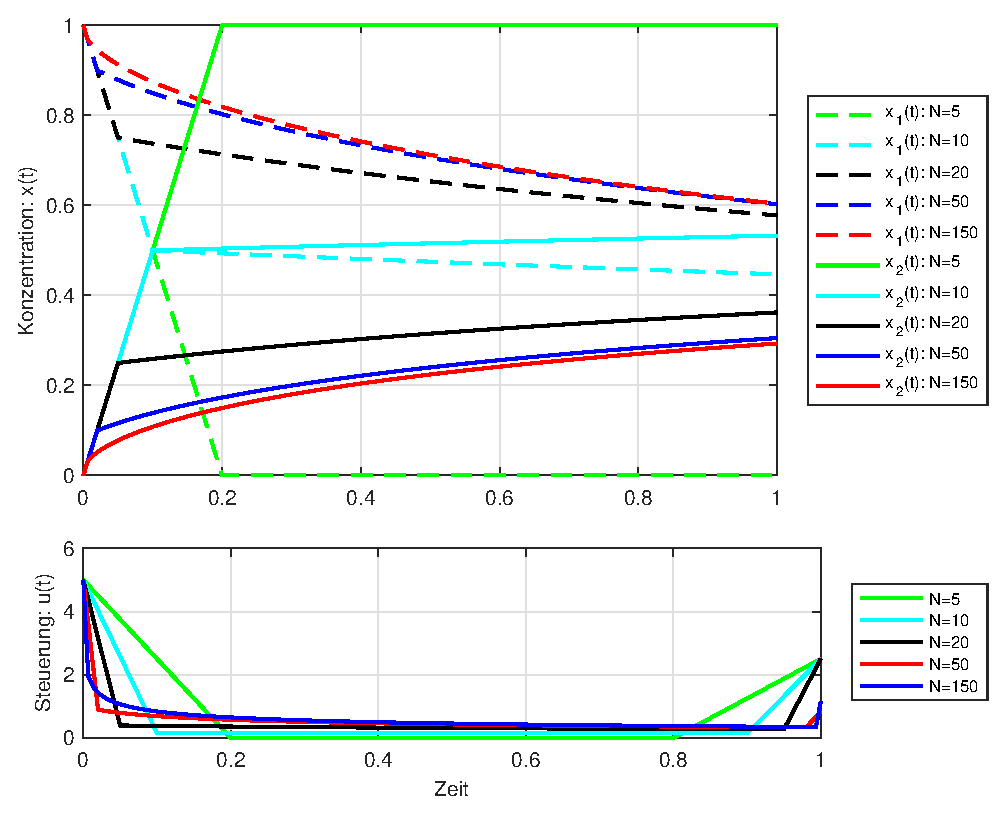
\includegraphics[width=.98\textwidth]{images/Expl_Result}
	\caption{Direktes Verfahren: Vollständige Euler-Diskretisierung}
	\label{fig:ExplEuler}
\end{figure}
\\Andere Beobachtungen können bei dem impliziten Radau2A-Verfahren gemacht werden (vgl. \autoref{fig:Radau2A}). Bereits ab $N \geq 20$ sind alle Lösungen fast identisch. Im Gegensatz zum Euler-Verfahren ist indes selbst eine physikalisch sinnvolle Lösung ab $N \geq 5$ erkennbar. Sowohl die Trajektorie von $x_1(t)$ und $x_2(t)$, als auch die berechnete optimale Steuerung $u(t)$ stimmen bereits bei einer großen Gitterweite mit den erwarteten Verläufen überein. Kleinere Ungenauigkeiten sind bei $N=5$ bzw. $N=10$ auf das gröbere Gitter zurückführen. Das bessere Verhalten des Radau2A-Verfahren bei einer kleineren Anzahl von Gitterpunkten lässt sich mit der höheren Konsistenz- und Konvergenzordnung begründen. Das Euler-Verfahren besitzt die Ordnung 1, das Radau2A-Verfahren hingegen die Ordnung 3.
\begin{figure}[h!]
	\centering
	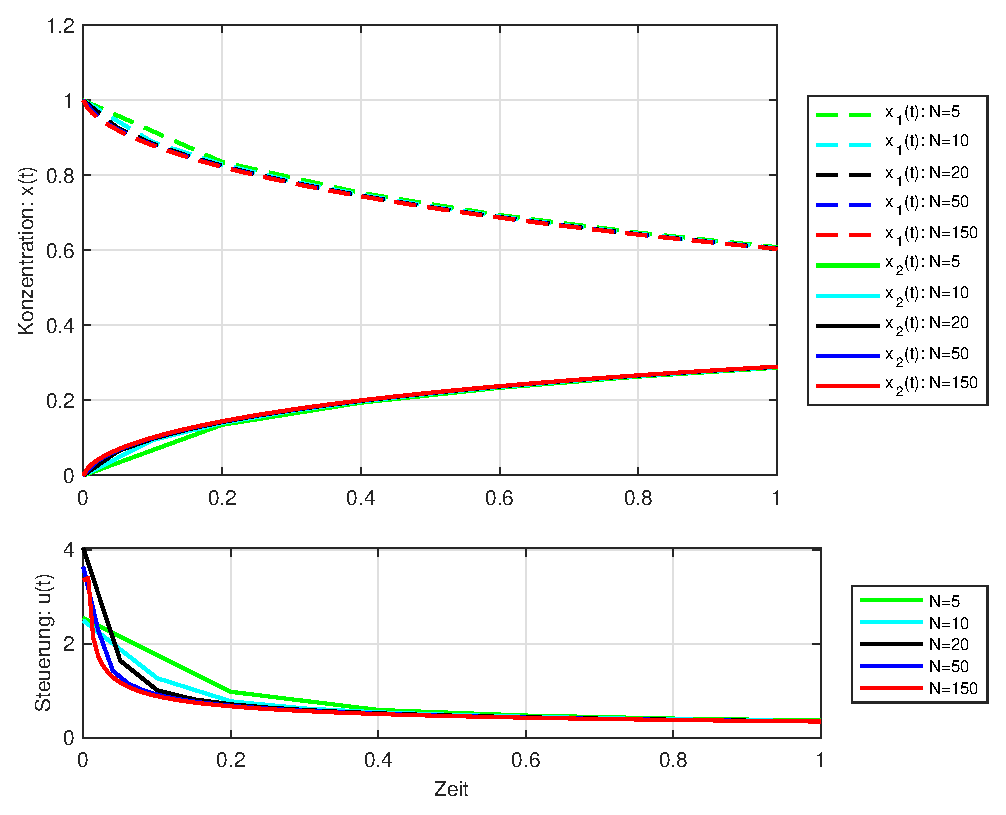
\includegraphics[width=.98\textwidth]{images/Radau2A_Result}
	\caption{Direktes Verfahren: Implizites Radau2A-Verfahren}
	\label{fig:Radau2A}
\end{figure}
\\Eine ebenfalls qualitativ sehr gute Lösung berechnet das Matlab-Verfahren \textit{ODE23s}, fast äquivalent zum Radau2A-Verfahren. Bereits bei einer sehr geringen Anzahl von Optimierungsstellen ($N=10$) ändert/ verbessert sich das Ergebnis mit einer Erhöhung der Stützstellen nicht mehr wesentlich. Ein möglicher Grund ist die adaptive Schrittweitensteuerung des Verfahrens. Zwischen zwei Optimierungsstellen $t^{(i)}$ und $t^{(i+1)}$ macht die vollständige Euler-Diskretisierung und das Radau2A-Verfahren nur einen Schritt. Das Verfahren \textit{ODE23s} jedoch passt die Schrittweite an und kann zwischen $t^{(i)}$ und $t^{(i+1)}$ noch Zwischenschritte einfügen, welche zwar nicht mit in die Optimierung eingehen, jedoch helfen die Dynamik besser zu approximieren. Die Betrachtung anderer Matlab-Verfahren, wie z.B. \textit{ODE45}, welches ebenfalls eine adaptive Schrittweitensteuerung besitzt und nicht für steife Probleme geeignet ist, lieferte ähnliche Ergebnisse und untermauert somit die Behauptung. Der Löser \textit{ODE23s} basiert auf einem Einschrittverfahren mit modifizierter Rosenbrock-Formel der Ordnung 2. \cite{ode23s}
\begin{figure}[h!]
	\centering
	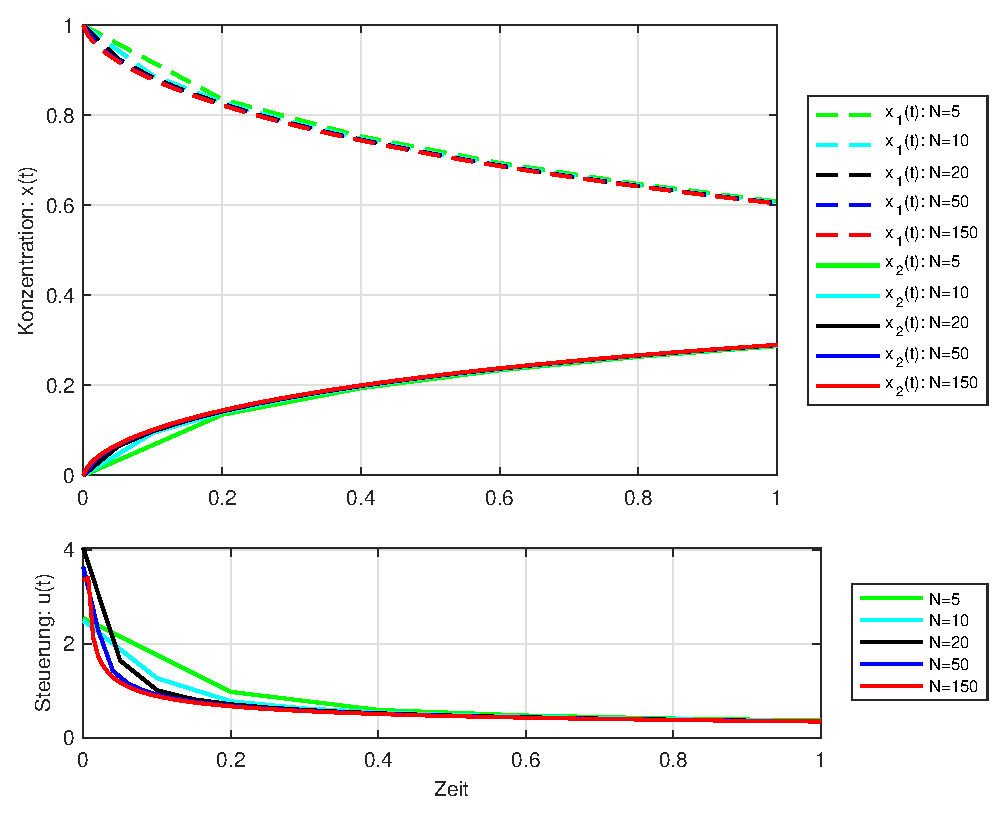
\includegraphics[width=.98\textwidth]{images/ODE23s_Result}
	\caption{Direktes Verfahren: \textit{ODE23s} Matlab-Verfahren)}
	\label{fig:ODE23s}
\end{figure}

\begin{figure}[h!]
	\centering
	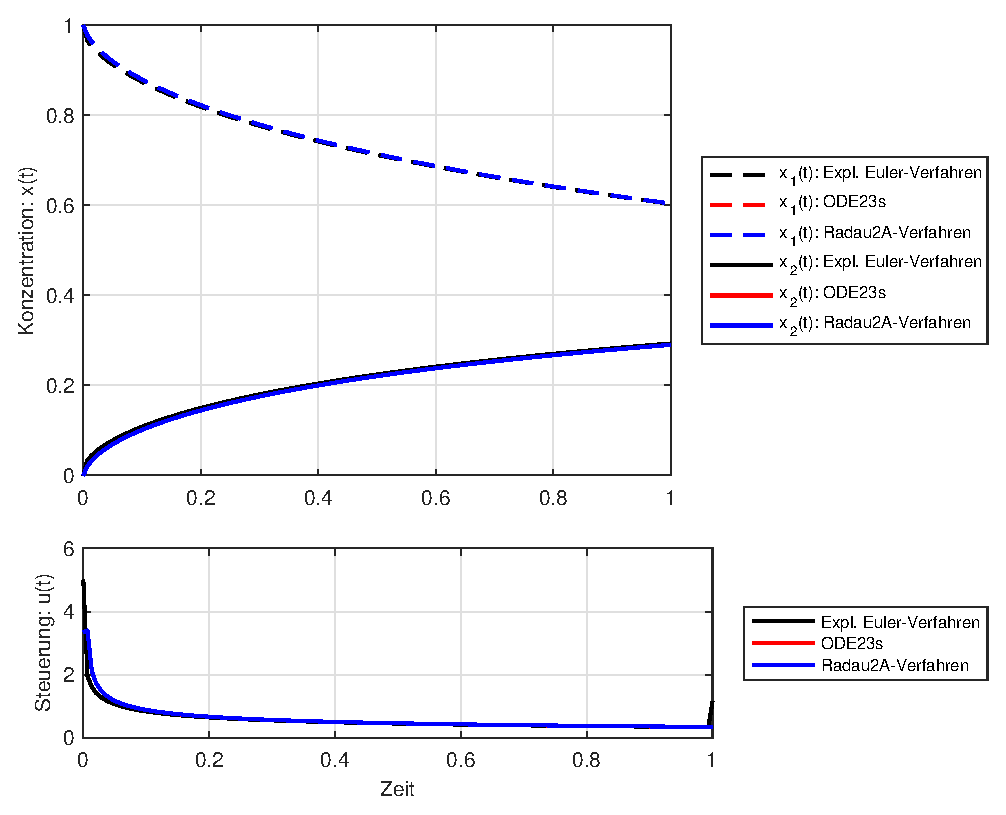
\includegraphics[width=.98\textwidth]{images/CompareDirect_Method}
	\caption{Direkte Verfahren: Vergleich}
	\label{fig:CompareDisk}
\end{figure}

Zusammenfassend lässt sich sagen, dass bei der entsprechenden Wahl von $N$ alle Verfahren sinnvolle Lösungen erzeugen. Die Konzentration von $x_1(t)$ wird kontinuierlich abgebaut und die von $x_2(t)$ gleichmäßig erhöht. Am Ende des Betrachtungszeitraum zeichnet sich ein chemisches Gleichgewicht ab, was in der Realität auch zu erwarten wäre.  Aus diesem Grund stabilisiert sich auch die Steuerung zum Ende hin. Des Weiteren liefern alle Verfahren ein ähnliches Ergebnis und liegen deshalb in \autoref{fig:CompareDisk} fast komplett übereinander.

\pagebreak

\section{Steifigkeitsanalyse}
Um die Behauptung aus \autoref{sec:ErgebnisseDisk} zu bestätigen, dass das System aus \autoref{ch:Aufgabe} nicht steif ist, wird eine vereinfacht Steifigkeitsanalyse durchgeführt. Im Allgemeinen wird ein lineares Anfangswertproblem (kurz: AWP) der Form
\begin{align}\label{eq:LinAWP}
	\dot{x}(t) = Ax+b, &&x(0) = x_0%\dot{x}(t) = f(t,x(t)), &&x(0) = x_0
\end{align}
als steif bezeichnet, wenn gilt :
\begin{align} \label{eq:Quotient}
	\Re(\lambda_i) <0, &&\max_{i,j} \frac{|\lambda_i|}{|\lambda_j|} \gg 1
\end{align}
Dabei stellen $\lambda_k$ die Eigenwerte der Matrix $A$ dar. Ist ein nichtlineares AWP zu untersuchen, dann muss zu jedem Zeitpunkt eine Taylor-Entwicklung 1. Ordnung durchgeführt und die Eigenwerte der Jacobi-Matrix in jedem Iterationsschritt einzeln betrachtet werden. Dies trifft auf das Problem aus \autoref{ch:Aufgabe} zu. Die Jacobi-Matrix für das DGL-System lautet:
\begin{align}
	\frac{\partial f(t,u(t),y(t))}{\partial y} = J_f(t,u(t),y(t)) = \left(\begin{array}{cccc}
		-u&u^2&0&0\\
		u&-3u^2&0&0\\
		0&0&u&-u\\
		0&0&-u^2&3u^2\\
	\end{array}\right)			
\end{align}
Entsprechend ergibt sich durch Einsetzen der Steuerung aus \autoref{fig:CompareDisk} der Verlauf des Quotienten (\ref{eq:Quotient}) in \autoref{fig:StiffAna}. Der Maximalwert beträgt ca. $23,56$ und ist somit zwar größer als $1$, jedoch nicht indem Maß, dass die Dynamik als steif anzusehen ist. Aus diesem Grund wird die Aussage aus \autoref{sec:ErgebnisseDisk} bestätigt, dass das System nicht steif ist.
\begin{figure}[h!]
	\centering
	\includegraphics[width=.55\textwidth]{images/StiffAna}
	\caption{Steifigkeitsanalyse: Quotient $\max_{i,j} \frac{|\lambda_i|}{|\lambda_j|}$ über Iterationsschritt $t^{(k)}$}
	\label{fig:StiffAna}
\end{figure}
In erster Linie bereitet das Phänomen der Steifheit expliziten Verfahren zur Lösung von gewöhnlichen Differentialgleichungen Probleme, sodass diese nicht konvergieren und ein instabiles Verhalten aufzeigen. Dies hat zur Folge, dass für die Lösung steifer Probleme implizite Verfahren zu bevorzugen sind, welche jedoch einen erhöhten Rechenaufwand aufweisen.  Da das hier vorliegende Problem hingegen nicht steif ist, liefern auch explizite Verfahren sinnvolle Lösungen und bieten den Vorteil des geringeren Berechnungsaufwandes.